\subsection{Batterij} \label{sec:battery}
In onderzoek \cite{BatteryComparison} is te zien dat Lithium-Polymeer batterijen (LiPo) een hoge energiedichtheid hebben in vergelijking met andere soorten batterijen. Er zijn andere batterijtechnologieën die een hogere energiedichtheid hebben. Deze zijn echter significant duurder, of hebben andere nadelige effecten \cite{BatteryComparison}. Hierdoor is voor de sensormodule een LiPo gekozen is als batterij. De spanning van een LiPo (1s) cel mag niet boven de 4.2 V of onder de 2.7 V komen \cite{BatteryComparison}.

\subsection{Voeding} \label{sec:voeding} 

%!! TODO: aai de kat, energy harvesting, spanning, batterij laden, beveiliging, stroom. 

De voedingsspanning is gekozen vanuit de maximale spanning die nodig is voor de ISFET sensor \cite{isfet}. Hieruit volgt een maximale systeemspanning van \qty{3.3}{\volt}. 


Zoals te lezen in \cref{sec:battery} is er gekozen voor LiPo batterij technologie. De batterij heeft een beveiliging voor beide op- en ontladen nodig. De celspanning moet omgezet worden naar systeemspanning van \qty{3.3}{\volt}. Dit wordt op 2 manieren gedaan, met een DC-DC buck-boost converter en een low dropout regelaar (LDO). De buck-boost is efficiënter dan de LDO. Een voordeel van de LDO is dat de spanningsrimpel veel lager is dan bij een buck-boost. Daarom wordt de LDO gebruikt voor het voeden van de analoge uitleesschakeling. De buck-boost gaat naar het digitale deel. Als een microcontroller goed ontkoppeld is dan maakt de spanningsrimpel niet uit voor de werking van de microcontroller. Daardoor is de hogere rimpel spanning van de buck-boost niet een probleem voor de microcontroller. De voeding is schematisch te zien in \cref{fig:voedingSchematisch}.

Voor energy harvesting is er een piëzo-elektrisch element gekozen. Een piëzo-elektrisch element kan mechanische trillingen omzetten in elektrische energie. De uitgang van een piëzo-elektrisch element kan gezien worden als een AC bron. Om deze AC bron te gebruiken, moet deze omgezet worden naar DC. Deze DC spanning kan gebruikt worden om de batterij mee op te laden. Dit wordt gedaan door middel van een gelijkrichter. Deze DC spanning is niet hetzelfde als de batterijspanning dus moet deze omgezet worden naar een veilige spanning, zodat de batterij ermee kan opladen.

\begin{figure}[ht]
    \centering 
    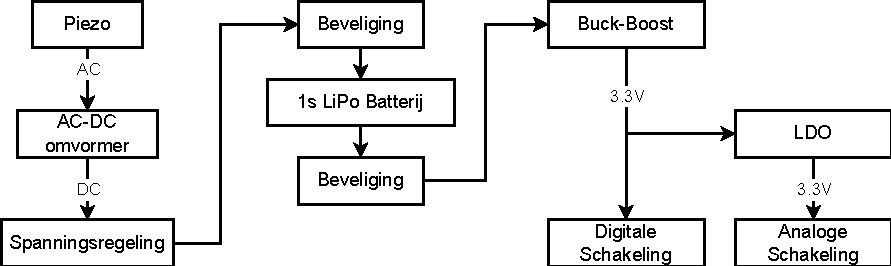
\includegraphics{voedingSchematisch.pdf}
    \caption{Voeding schematisch}
    \label{fig:voedingSchematisch}
\end{figure}



\subsection{Energie budget}
Voor het energiebudget zijn de waardes uit \cref{tab:energieBudgetEstimatie} gekozen. Deze waardes zijn ruim boven de theoretisch berekende minimum waardes liggen. Met deze waardes ligt het totale systeemverbruik nog steeds onder de in \cref{tab:systemSpecs} gespecificeerde \qty{10}{\milli\watt}.


\begin{table}[ht]
    \centering
    \begin{tabular}{l|l}
        Func. blok          & Vermogen [mW] \\
        \hline                              
        Reken $U_{GS}\rightarrow$pH & 0.6   \\
        ADC                 & 1             \\
        AA-filter           & 0.2           \\
        Meet $U_{GS}$       & 0.2           \\
        Zenden              & 5             \\
        Oplader             & 0.5           \\
        Beveiliging         & 0.5           \\
        Spanningsregeling   & 1             \\ 
        \hline
        \hline
        Totaal              & 9
        
    \end{tabular}
    \caption{Energie budget}
    \label{tab:energieBudgetEstimatie}
\end{table}


